
\documentclass[ letterpaper, titlepage, fleqn]{article}

\usepackage[utf8]{inputenc}
\usepackage[slovene]{babel}
\usepackage[margin=60px]{geometry}
\usepackage{amsmath}
\usepackage{amssymb}
\usepackage{enumerate}
\usepackage{graphicx}
\usepackage{mathrsfs}
\usepackage{mathabx}
\usepackage{faktor}
\usepackage{bbm}

\setlength\parindent{0pt}

\newcommand{\R}{\mathbb R}
\newcommand{\N}{\mathbb N}
\newcommand{\Z}{\mathbb Z}
\newcommand{\C}{\mathbb C}
\newcommand{\Q}{\mathbb Q}
\newcommand{\F}{\mathscr{F}}
\newcommand{\E}{\mathbb E}
\newcommand{\FF}{\mathbb F}
\newcommand{\K}{\mathbb K}
\newcommand{\D}{\mathbb D}
\newcommand{\J}{\mathscr J}
\newcommand{\T}{\mathscr T}
\newcommand{\LL}{\mathscr L}

\newcommand{\mul}{\text{mul}}
\newcommand{\add}{\text{add}}
\newcommand{\abs}{\text{abs}}
\newcommand{\aph}{\text{@}}
\newcommand{\primea}{\textsc{\char13}}
\newcommand{\norm}[1]{\left\lVert#1\right\rVert}
\newcommand{\adjscalar}[1]{\left\langle\;#1\;\right\rangle}
\newcommand{\scalar}[1]{\langle\;#1\;\rangle}
\newcommand{\zeroradical}{\sqrt{0}}
\newcommand{\Bin}{\text{Bin}}
\newcommand{\id}{\text{id}}
\newcommand{\ind}{\mathbbm{1}}

\providecommand{\floor}[1]{\left \lfloor #1 \right \rfloor }

\begin{document}

\section{1}

\subsection{}
Če zapišemo gostote v eksponentni obliki, dobimo
$$f(x; a,b) = \frac{b^a}{\Gamma(a)} \exp(-\scalar{(a+1, b), (\ln(x), 1/x)}) \cdot \ind_{(0,\infty)}(x),$$
torej po Fisher-Neymanovem faktorizacijskem izreku dobimo, da je
$$T(x) = (\ln(x), 1/x)$$
zadostna statistika za ta model. Ker je to eksponenten model s polnim rangom, pa je $T$ tudi kompletna.

\subsection{}
Ker smo v parametričnem modelu z zvezno odvedljivimi gostotami, lahko iščemo stacionarne točke gostot 
z logaritmično enačbo verjetja. Računamo
\begin{equation*}
\begin{aligned}
&l(a,b) := \ln(f(x; a,b)) = a\ln(b) - \ln(\Gamma(a)) - (a+1)\ln(x) - \frac{b}{x} \\
&\frac{\partial l}{\partial a}(a,b) = \ln(b) - \frac{\Gamma'(a)}{\Gamma(a)} - \ln(x) \\
&\frac{\partial l}{\partial b}(a,b) = \frac{a}{b} - \frac{1}{x}.
\end{aligned}
\end{equation*}
Zapišemo lahko logaritemsko enačbo verjetja
$$\ln(b) - \frac{\Gamma'(a)}{\Gamma(a)} - \ln(x) = \frac{a}{b} - \frac{1}{x} = 0,$$
iz česar takoj dobimo $b = ax$, za drugo enačbo pa potem sledi, da rešujemo
$$\Psi(a) := \ln(a) - \frac{\Gamma'(a)}{\Gamma(a)} = 0.$$
Po posledici Bernsteinovega izreka o monotonih funkcijah velja, da je za $x > 0$
$$\Psi(x) - \frac{1}{2x} > 0,$$
torej naša funkcija nima ničel in zato cenilka po metodi največjega verjetja ne obstaja.

\subsection{}
Naj bo $P_{(a,b)}$ mera, inducirana z gostoto $f(\cdot; a,b)$. Za $k\in\N$ velja
\begin{equation*}
m_k := P_{(a,b)}[\id^k] = \int_0^\infty \frac{b^a}{\Gamma(a)} x^{-a-1} e^{-b/x} x^k dx
= \frac{b^a}{\Gamma(a)} \frac{\Gamma(a-k)}{b^{a-k}} \int_0^\infty \frac{b^{a-k}}{\Gamma(a-k)} x^{-(a-k)-1} e^{-b/x} dx 
= b^k \frac{\Gamma(a-k)}{\Gamma(a)}.
\end{equation*}
Označimo
$$
\hat{b}(x_1, x_2, x_3) := \left(\frac{x_1}{x_2} - \frac{x_2}{x_3}\right)^{-1} \quad \text{in} \quad
\hat{a}(x_1, x_2, x_3) := \frac{\hat{b}(x_1,x_2,x_3)}{x_1} + 1.
$$
Opazimo, da je $\hat{b}(m_1,m_2,m_3) = b$ in $\hat{a}(m_1,m_2,m_3) = a$,
torej dobimo zaporedje cenilk po metodi momentov
$$(\hat{a}, \hat{b}) \circ (\hat{m_1^n}, \hat{m_2^n}, \hat{m_3^n}),$$
kjer je
$$\hat{m_k^n}(x) = \frac{1}{n} \sum_{i=1}^n x_i^ k.$$
Ker je $g = (\hat{a}, \hat{b})$ zvezna na $\R_+^3$, je ta cenilka dosledna. Sicer pa je $g$ za analizo še kar zahtevna preslikava in zato je izračun konkretne porazdelitve ali katerega od momentov težek problem.


\subsection{}
Označimo $X^{(n)} := (X_1, \dots, X_n) \sim P_{(a,b)}^{\times n}$ in NEP vektorje $Y_i := (X_i, X_i^2, X_i^3)$ . Dalje
$$
M_n := (\hat{m_1^n}, \hat{m_2^n}, \hat{m_3^n}) \quad \text{in} \quad
\hat{\vartheta}_n := g \circ M_n.
$$
Po centralnem limitnem izreku velja
$$\sqrt{n} \cdot \left(M_n(X^{(n)}) - \mu \right) = \sqrt{n} \cdot\left(\frac{1}{n} \sum_{i=1}^n Y_i - \mu\right) \xrightarrow[n\to\infty]{D} N(0, \Sigma),$$
kjer je $\mu$ pričakovana vrednost, $\Sigma$ pa variančno-kovariančna matrika vektorjev $Y_i$.
Potem nam metoda delta skupaj s Cramer-Woldovim pravilom zagotovi
$$\sqrt{n} \cdot (\hat{\vartheta}_n(X^{(n)}) - \vartheta) = \sqrt{n} \cdot (g(M_n(X^{(n)})) - g(\mu)) \xrightarrow[n\to\infty]{D} N(0, \J_g(\mu) \Sigma \J_g(\mu)^T),$$
saj je očitno $\mu = [m_1, m_2, m_3]^T$.

\subsection{}
Enostavno izračunamo
$$\Sigma = 
\begin{bmatrix}
m_2 - m_1^2 & m_3 - m_1m_2 & m_4 - m_1m_3 \\
m_3 - m_1m_2 & m_4 - m_2^2 & m_5 - m_2m_3 \\
m_4 - m_1m_3 & m_5 - m_2m_3 & m_6 - m_3^2 
\end{bmatrix}
$$
in označimo
$$A := \J_g(\mu) \Sigma \J_g(\mu)^T.$$
Definirajmo sedaj zaporedje cenilk $\hat{A}_n$ tako, da zamenjamo v $A$  elemente $m_i$ z $\hat{m_i^n}$.
Potem uporabimo Sluckyjev izrek, zveznost korena ter inverza (simetrične, pozitivno definitne) matrike in malo ocenimo
$$\pi_n(X^{(n)}, \vartheta) := \sqrt{n} \cdot \hat{A}_n^{-1/2}(X^{(n)}) \left(\hat{\vartheta}_n(X^{(n)}) - \vartheta\right) \xrightarrow[n\to\infty]{D} N(0, I).$$
Naj bo $B \subset \R^2$ neka množica, ki zadošča
$$P(\pi_n(X^{(n)}, \vartheta) \in B) \approx N(0,I)(B) = 1 - \alpha.$$
Sledi
$$P(\pi_n(X^{(n)}), \vartheta) \in B) = P_{\vartheta}^{\times n}(\hat{\vartheta}_n - \vartheta \in \hat{A}_n^{1/2})\left(B\right) / \sqrt{n}) = P_{\vartheta}^{\times n}(\vartheta \in \hat{\vartheta}_n - \hat{A}_n^{1/2}\left(B\right) / \sqrt{n}),$$
torej je območje zaupanja za $\vartheta$ enako
$$\hat{\vartheta}_n(X^{(n)}) - \hat{A}_n^{1/2}(X^{(n)})\left(B\right) / \sqrt{n}.$$
Vprašanje izbire množice $B$ lahko rešimo s predpostavko, da je to zaprta krogla s središčem v $0$ v neki normirani metriki, 
s čimer se verjetno da dokazati enoličnost njenega radija. Če vzamemo normo $\norm{.}_2$, dobimo, da je območje zaupanja enako elipsi
$$\hat{\vartheta}_n + Q_n \sqrt{\Lambda}_n B / \sqrt{n},$$
kjer je $\hat{A}_n = Q_n \Lambda_n Q_n^T$ Schurova forma. Sicer pa je bolj priročno vzeti normo $\norm{.}_\infty$, saj lahko izrazimo 
\begin{equation*}
N(0,I)\left([-r,r]^2\right) = \left(N(0,1)([-r,r])\right)^2 = 1 - \alpha 
\end{equation*}
in dobimo, da je $r$ enak zgornjemu $((1 - \sqrt{1-\alpha})/2)$-percentilu porazdelitve $N(0,1)$. Podobno kot pri elipsi, tu dobimo paralelogram. Spodaj je prikazana realizacija tega paralelograma glede na dane podatke.
\begin{center}
\begin{figure}[h]
\begin{center}
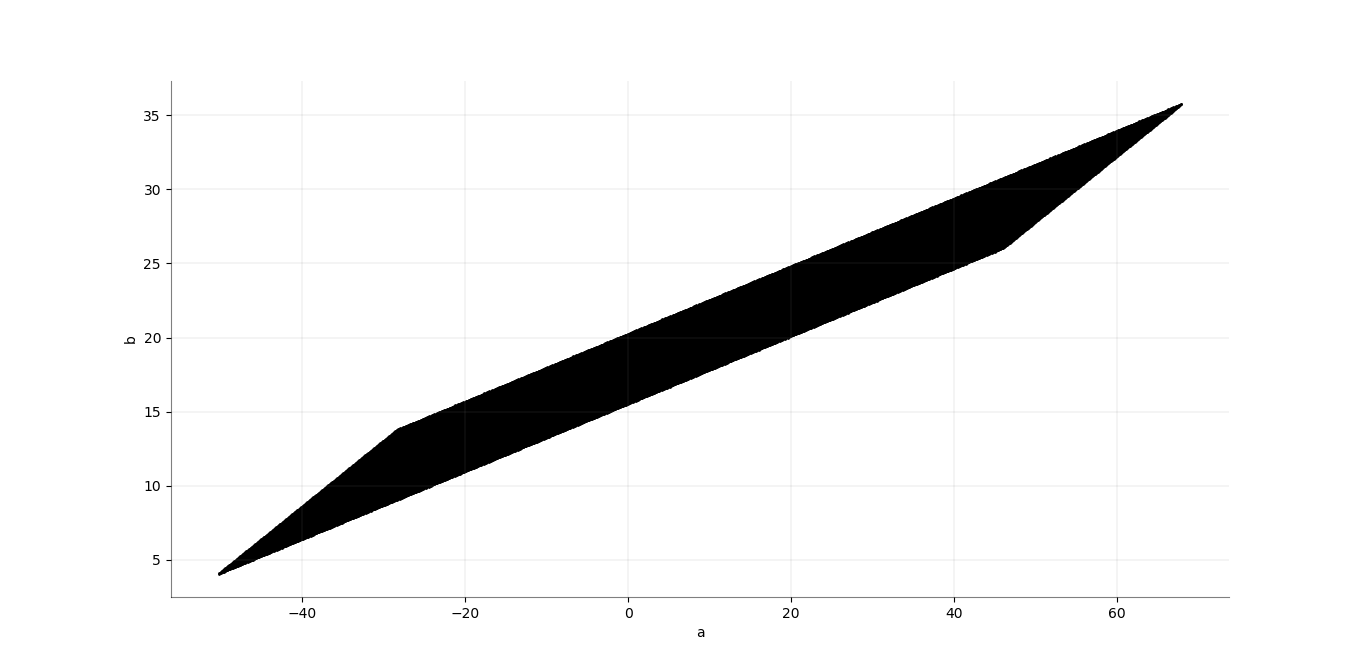
\includegraphics[width=15cm]{graphics/ConfidenceParalelogram.png}
\end{center}
\end{figure}
\end{center}


\section{2}
Naj bo $(X_i, \dots, X_n) \sim N(\mu, \sigma_0)^{\times n}$ za $i=1,\dots,n$ in $\sigma_0 \in \R^+$, $n\in\N$ fiksna. Po Rao-Blackwellovem izreku lahko najdemo NCEND kot pogojno upanje nepristranske cenilke $\ind_{\{X_1 \leq 5\}}$  pogojno na kompletno in zadostno statistiko
$$\bar{X} = \frac{1}{n} \sum_{i=1}^n X_i.$$
Označimo $Y = \bar{X} - \mu$ in definirajmo
$$\tilde{X} = X_1 - \zeta Y, \text{ kjer je } \zeta = P[X_1Y] / \sigma(Y)^2.$$
Zanjo velja
$$P[\tilde{X}Y] = P[X_1Y] - \zeta P[Y^2] = 0,$$
torej sta $\tilde{X}$ in $Y$ nekorelirani, ker pa sta normalni, sta tudi neodvisni. 
Sedaj lahko zapišemo
\begin{equation*}
\begin{aligned}
P[\ind_{\{X_1 \leq 5\}} \mid \bar{X} = t] &= P(X_1 \leq 5 \mid \bar{X} = t) 
= P(\tilde{X} + \zeta Y \leq 5 \mid Y + \mu = t) = P(\tilde{X} + \zeta (t - \mu) \leq 5) \\
&= P(X_1 - \zeta (\bar{X} - \mu) + \zeta(t - \mu) \leq 5) = P(X_1 - \zeta \bar{X} \leq 5 - \zeta t).
\end{aligned}
\end{equation*}
Konkretno:
\begin{equation*}
P[X_1Y] = P[(\sigma_0 Z_1 + \mu)Y] = P[\sigma_0 Z_1 Y] = P[\sigma_0 Z_1 \sum_{i=1}^n \frac{\sigma_0}{n} Z_i] = \frac{\sigma_0^2}{n} P[Z_1^2]  = \frac{\sigma^2}{n},
\end{equation*}
torej skupaj z dejstvom $\sigma(Y) = \sigma_0 / \sqrt{n}$ dobimo $\zeta = n$ in NCEND
$$U(\bar{x}) = P(\sigma_0 (1 + 1/\sqrt{n})Z \leq 5 - \bar{x}) = \Phi\left(\frac{5 - \bar{x}}{\sigma_0(1 + 1/\sqrt{n})}\right)$$

\section{3}
\subsection{}
Fiksirajmo $n\in\N$ in označimo s $P_\vartheta$ $n$-razsežno produktno mero mere, inducirane z gostoto $f(\_, \vartheta)$. Ker je
\begin{equation*}
f(k_1, \dots, k_n; \vartheta) = \prod_{i=1}^n f(k_i; \vartheta) =  (-\ln(1-\vartheta))^{-n} \left(\prod_{i=1}^n k_i^{-1}\right) \exp\left(\ln(\vartheta) \sum_{i=1}^n k_i\right)
\end{equation*}
in $\ln((0,1))  = (-\infty, 0) \in \T_{EVK} \smallsetminus \{\emptyset\}$, je to eksponentni model s polnim rangom, 
torej dobimo kompletno zadostno statistiko 
$$T(k_1, \dots, k_n) = \sum_{i=1}^n k_i.$$

\subsection{}
Ker imamo eksponenten model s funkcijo $Q \equiv \ln$, ki je strogo naraščajoča na $(0,1)$, lahko uporabimo Neuman-Pearsonovo
lemo za konstrukcijo enakomerno najmočnejših randomiziranih preizkusov. 
Ker ima model druge momente, si lahko pomagamo tudi z normalnimi aproksimacijami (asimptotično normalnostjo).

\subsection{}
Poskušajmo postopati z Neuman-Pearsonovo lemo. Označimo torej $\vartheta_0 = 0.7$ in $\alpha = 0.05$.
Potem imamo enakomerno najmočnejši randomiziran preizkus za $\vartheta \leq \vartheta_0$ proti alternativi
$\vartheta > \vartheta_0$ v obliki
$$
\phi(k_1, \dots, k_n)= 
\begin{cases}
1 \mid & T(k_1, \dots, k_n) > C \\
\gamma \mid &  T(k_1, \dots, k_n) = C \\
0 \mid &  T(k_1, \dots, k_n) < C
\end{cases},
$$
kjer določimo $C \in\N$ in $\gamma \in [0,1)$ enolično s pogojem
$$\beta(\vartheta_0) = P_{\vartheta_0}[\Phi] = P_{\vartheta_0}(T > C) + \gamma P_{\vartheta_0}(T = C) = \alpha.$$
Idealno bi bilo imeti porazdelitev $T$, a ta vključuje izračun vsot, ki v splošnem nimajo zaključene oblike ($\sum_{k=1}^d \vartheta^k / k$). Če bi imeli dovolj majhen vzorec, to tudi ne bi bil problem, saj bi izračunali posamezne vrednosti gostote $T$ z brute-force varianto. Ker pa je vzorec velikosti $n=50$ relativno velik, tega ne moremo izvesti. Lahko pa zato $T$ aproksimiramo z normalno porazdelitvijo (po CLI). Računamo
\begin{equation*}
\begin{aligned}
\mu_\vartheta 
&:= P_{\vartheta}[\id] 
= -\frac{1}{\ln(1 - \vartheta)} \sum_{k\in\N} \vartheta^k 
= - \frac{1}{\ln(1 - \vartheta)}\frac{\vartheta}{(1 - \vartheta)}  \\
\sigma_\vartheta^2 
&:= V_{\vartheta}[\id] 
= P_{\vartheta}[\id^2] - P_{\vartheta}[\id]^2 
= -\frac{1}{\ln(1 - \vartheta)} \sum_{k\in\N} k\vartheta^k - \mu_\vartheta^2 
= -\frac{1}{\ln(1 - \vartheta)} \frac{\vartheta}{(1-\vartheta)^2} - \mu_\vartheta^2.
\end{aligned}
\end{equation*}
Označimo produktno mero
$$\tilde{P}_\vartheta := N(\mu_\vartheta, \sigma_\vartheta^2)^{\times n}.$$
Sedaj lahko ocenimo gostoto statistike $T$ kot
$$P_\vartheta(T = k) \approx \tilde{P}_\vartheta(T \leq k) - \tilde{P}_\vartheta(T \leq k-1).$$
Aproksimirajmo:
\begin{equation*}
\begin{aligned}
\alpha &= 1 - P_{\vartheta_0}(T \leq C) + \gamma P_{\vartheta_0}(T = C) \\
&\approx 1 - \tilde{P}_{\vartheta_0}(T \leq C) + \gamma \tilde{P}_{\vartheta_0}(T \in [C-1, C]) \\
&= 1 - \Phi\left(\frac{C/n - \mu_{\vartheta_0}}{\sigma_{\vartheta_0} / \sqrt{n}}\right) + \gamma\left(
\Phi\left(\frac{C/n - \mu_{\vartheta_0}}{\sigma_{\vartheta_0} / \sqrt{n}}\right) -
\Phi\left(\frac{(C-1)/n - \mu_{\vartheta_0}}{\sigma_{\vartheta_0} / \sqrt{n}}\right)
\right).
\end{aligned}
\end{equation*}
Vzamemo prvi $C\in\N$, za katerega je 
$$\gamma = \frac{\alpha +
\Phi\left(\frac{C/n - \mu_{\vartheta_0}}{\sigma_{\vartheta_0} / \sqrt{n}}\right) - 1}
{\Phi\left(\frac{C/n - \mu_{\vartheta_0}}{\sigma_{\vartheta_0} / \sqrt{n}}\right) -
\Phi\left(\frac{(C-1)/n - \mu_{\vartheta_0}}{\sigma_{\vartheta_0} / \sqrt{n}}\right)} \in [0,1).$$
Dobimo $C = 117$ in $\gamma \approx 0.9705$. Na spodnji sliki je prikazana funkcija moči dobljenega testa,
kjer so vrednosti spet aproksimirane z normalno porazdelitvijo.
\begin{center}
\begin{figure}[h]
\begin{center}
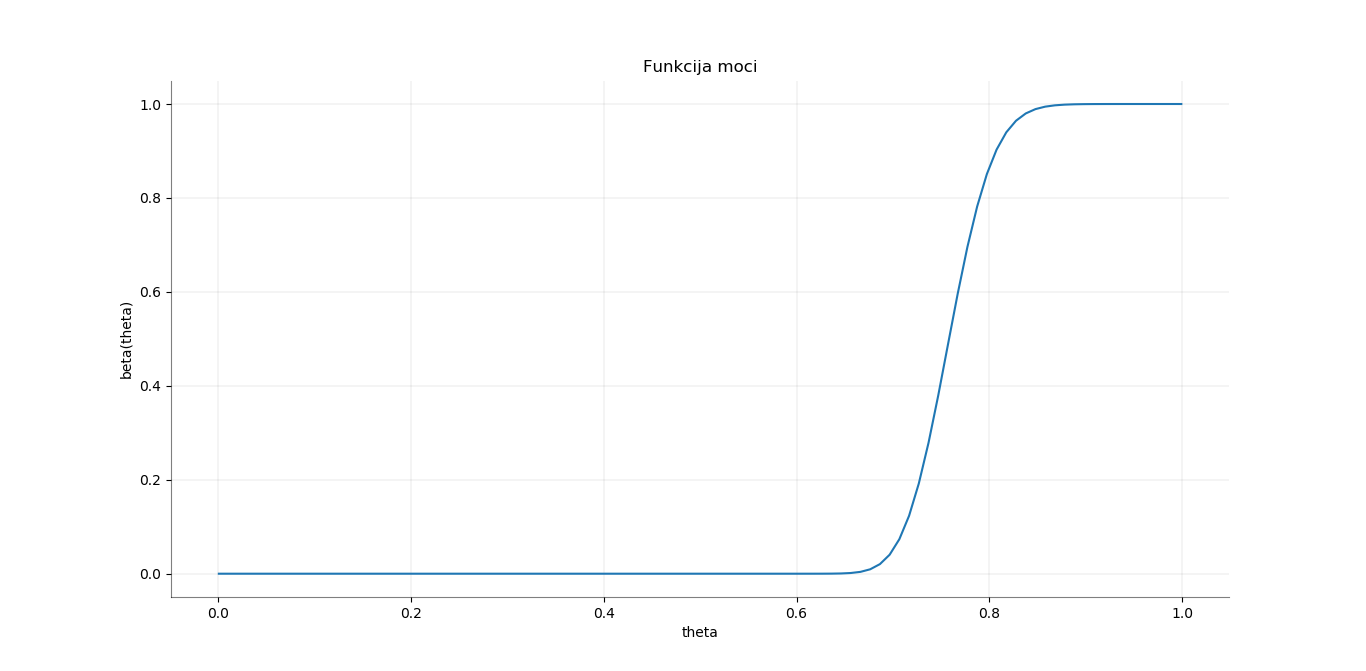
\includegraphics[width=13cm]{graphics/FunkcijaMoci.png}
\end{center}
\end{figure}
\end{center}

\subsection{}
Najprej nas zanima, če je za dani $x$ preslikava $f(x, \vartheta)$ monotona v odvisnosti od $\vartheta$. Ker dobimo
$$\frac{\partial f}{\partial\vartheta} (k, \vartheta) = -\frac{\vartheta^k}{k\ln(1-\vartheta)} \left(\frac{1}{(1-\vartheta)\ln(1-\vartheta)} + \frac{1}{\ln(\vartheta)}\right) < 0,$$
sledi, da je preslikava padajoča. Iz tega sledi, da je padajoča $F_\vartheta$ in zato tudi $F_{T; \vartheta}$. Vzamemo $\alpha_1 = \alpha_2 = \alpha/2$ in realiziramo interval $[0.5215, 1)$, kjer so bile vse vrednosti spet aproksimirane normalno.

\section{}
\subsection{}
Spet fiksirajmo $n\in\N$ in označimo $P_{p_0} = \text{Ber}(p_0)^{\times n}$ ter
$T(x_1, \dots, x_n) = \sum_{i=1}^n x_i.$
Neuman-Pearsonov test za hipotezo $p = p_0$ proti alternativi ima obliko
$$
\phi(x)= 
\begin{cases}
1 &\mid T(x) \in (C_1(p_0), C_2(p_0)) \\
\gamma_j(p_0)  &\mid  T(x) = C_j(p_0) \\
0 &\mid  T(x) \notin [C_1(p_0), C_2(p_0)]
\end{cases},
$$
kjer so vrednosti $C_j(p_0)$, $\gamma_j(p_0)$ določene z zahtevo
$$P_{p_0}[\phi_{p_0}] = \alpha \quad \text{in} \quad \frac{d}{dp_0} P_{p_0}[\phi_{p_0}] = 0.$$
Izračunamo 
\begin{equation*}
\begin{aligned}
P_{p_0}[\phi_{p_0}] &= P_{p_0}(T< C_1(p_0)) + P_{p_0}(T > C_2(p_0)) 
+ \gamma_1(p_0) P_{p_0}(T = C_1(p_0)) + \gamma_2(p_0) P_{p_0}(T = C_2(p_0)) \\
&= 1 - \sum_{i=C_1(p_0)}^{C_2(p_0)} \binom{n}{i} p_0^i (1-p_0)^{n-i}
+ \sum_{i\in\{1,2\}} \gamma_i(p_0) \binom{n}{C_i(p_0)} p_0^{C_i(p_0)} (1-p_0)^{n -C_i(p_0)}
\end{aligned}
\end{equation*}
in
\begin{equation*}
\begin{aligned}
\frac{d}{dp_0}& P_{p_0}[\phi_{p_0}] = 
- \sum_{i=C_1(p_0)}^{C_2(p_0)} \binom{n}{i}\left(i p_0^{i-1} (1-p_0)^{n-i} - (n-i) p_0^i (1-p_0)^{n-i-1}\right) + \\
& + \sum_{i\in\{1,2\}} \gamma_i(p_0) \binom{n}{C_i(p_0)} \left(C_i(p_0) p_0^{C_i(p_0-1)} (1-p_0)^{n -C_i(p_0)} -
(n-C_i(p_0)) p_0^{C_i(p_0-1)} (1-p_0)^{n-C_i(p_0)-1}\right).
\end{aligned}
\end{equation*}
Testiramo vse $0 \leq C_1(p_0) < n$ in $C_1(p_0) < C_2(p_0) \leq n$ in na vsaki iteraciji rešimo sistem dveh linearnih enačb za $\gamma_i(p_0)$. Vrnemo prve vrednosti, pri katerih velja $0 \leq \gamma_i(p_0) < 1$ za $i=1,2$.
\begin{center}
\begin{figure}[h]
\begin{center}
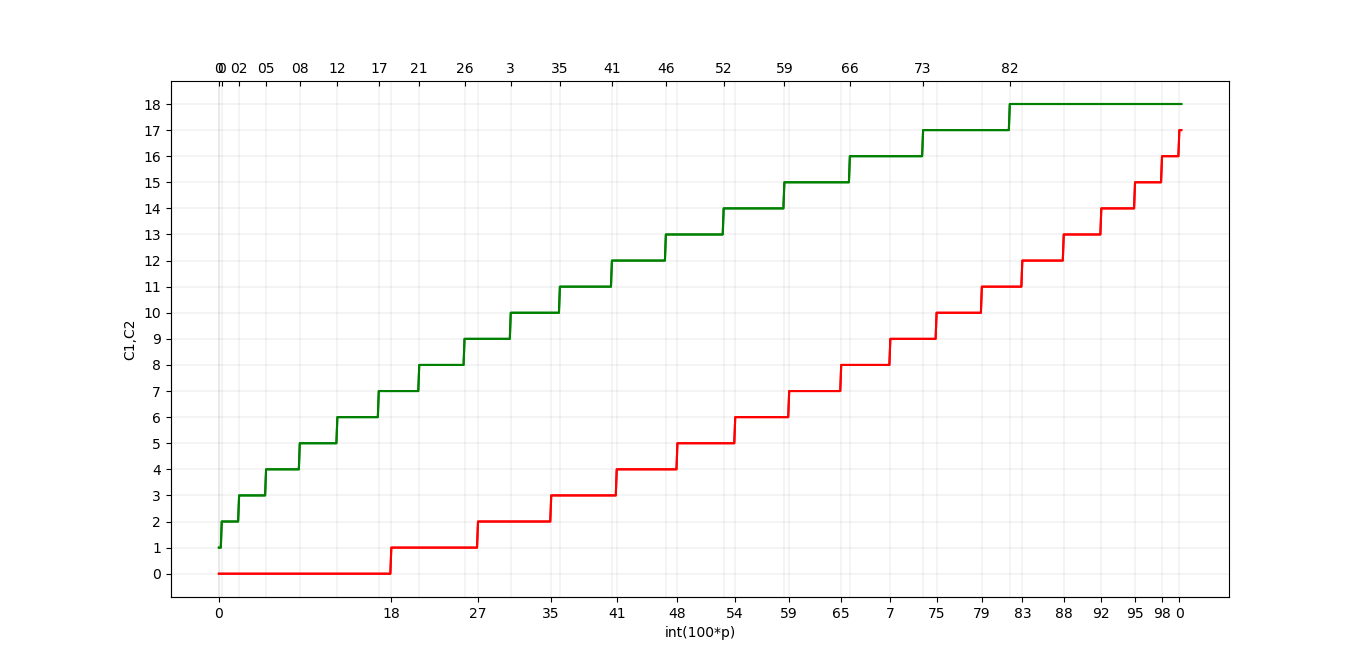
\includegraphics[width=15cm]{graphics/C1C2_18.png}
\caption{$C_1(p)$ in $C_2(p)$  na diskretizaciji $(0,1)$ na $1000$ točkah za $n=18$.}
\end{center}
\end{figure}
\end{center}

Za interval zaupanja definiramo
$$I(T(x)) := \{p \in (0,1) \mid \phi_p(x) < 1\} = \{p \in (0,1) \mid T(x) \in [C_1(p), C_2(p)]\}.$$
Za vsak $k=0,1,\dots,n$ bomo vzeli vse $p$ na neki diskretizaciji $(0,1)$, ki so v $I(k)$. Spodnja tabela prikazuje aproksimacijo $I\circ T$ pri delitvi intervala (0,1) na $1000$ delov, z zaokrožitvijo krajišč intervala na $3$ decimalna mesta.
\begin{center}
\begin{tabular}{ |l|l| }
\hline
$k$ & $I(k)$ \\
\hline
$0$ & $ (0, 0.18]$ \\
$1$ & $(0, 0.27]$ \\
$2$ & $[0.004, 0.346]$ \\
$3$ & $[0.022, 0.414]$ \\
$4$ & $[0.05, 0.477]$ \\
$5$ & $[0.085, 0.536]$ \\
$6$ & $[0.124, 0.592]$ \\
$7$ & $[0.167, 0.646]$ \\
$8$ & $[0.209, 0.697]$ \\
$9$ & $[0.256, 0.745]$ \\
$10$ & $[0.304, 0.792]$ \\
$11$ & $[0.355, 0.834]$ \\
$12$ & $[0.409, 0.877]$ \\
$13$ & $[0.465, 0.916]$ \\
$14$ & $[0.524, 0.951]$ \\
$15$ & $[0.587, 0.979]$ \\
$16$ & $[0.655, 0.997]$ \\
$17$ & $[0.731, 1)$ \\
$18$ & $[0.821, 1)$ \\
\hline
\end{tabular}
\end{center}

\subsection{}
Zaokroženo na $4$ decimalna mesta dobimo $\gamma_1(0.72) \approx 0.1787$ in $\gamma_2(0.72) \approx 0.6852$.

\subsection{}
\begin{center}
\begin{figure}[h]
\begin{center}
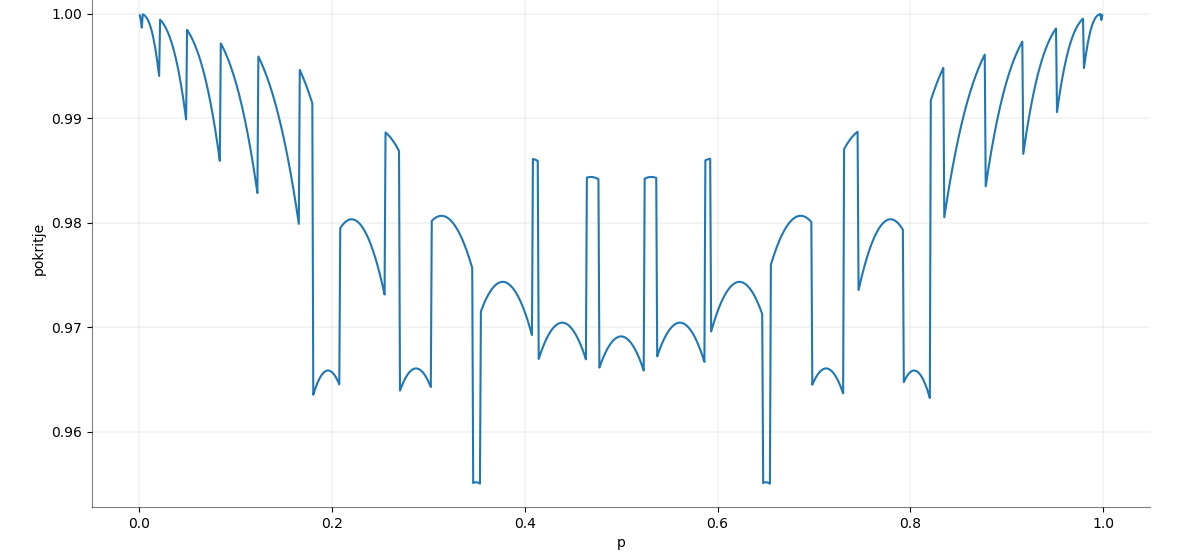
\includegraphics[width=15cm]{graphics/Pokritje.png}
\end{center}
\end{figure}
\end{center}
Ocena minimuma vrednosti na zgornjem grafu je $0.95502$, kar je naša ocena za koeficient zaupanja.

\subsection{}
Program nam vrne
$$C_1 = 15 \quad C_2 = 24 \quad \gamma_1 \approx 0.6922 \quad \gamma_2 \approx 0.0029$$

\subsection{}
\begin{center}
\begin{figure}[h]
\begin{center}
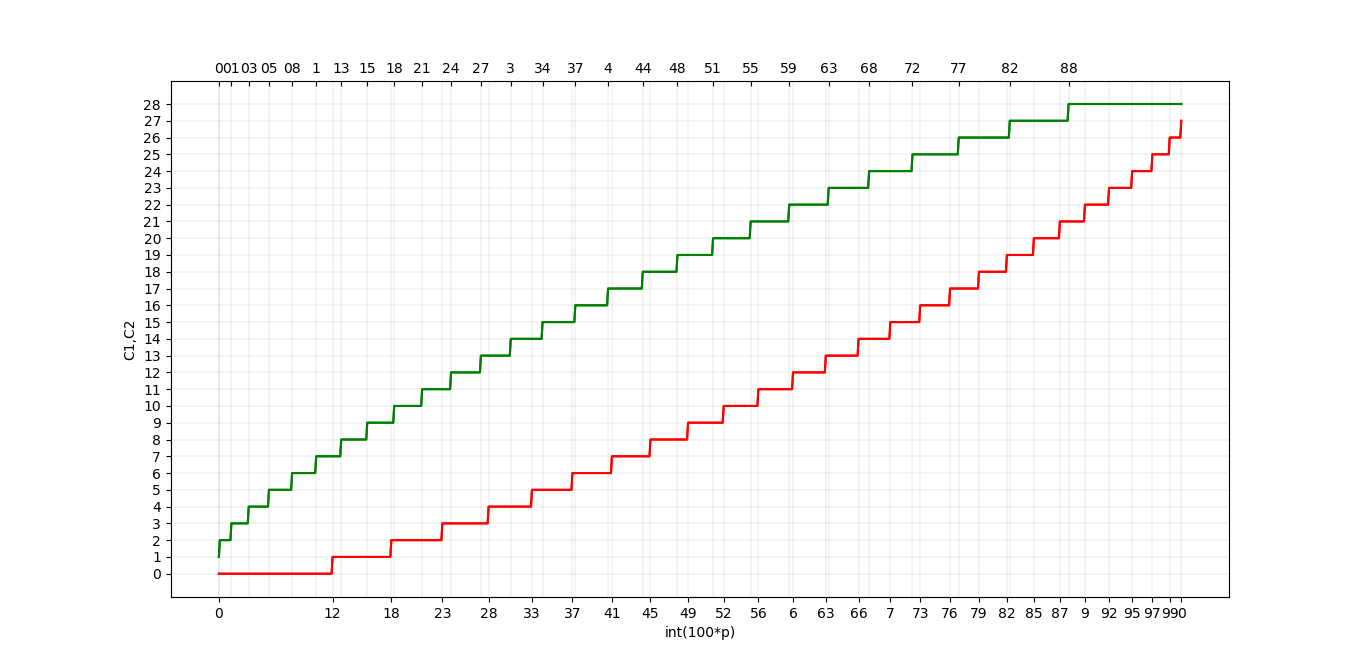
\includegraphics[width=15cm]{graphics/C1C2_28.png}
\caption{$C_1(p)$ in $C_2(p)$  na diskretizaciji $(0,1)$ na $1000$ točkah za $n=28$}
\end{center}
\end{figure}
\end{center}

\section{}
Označimo $p = (p_0, \dots, p_3)$ in
$$
P_p = \left(
\begin{array}{ll}
\xi_0 \quad \xi_1 \quad \xi_2 \quad \xi_3 \\
p_0 \quad p_1 \quad p_2 \quad p_3 \\
\end{array}
\right).
$$
Vemo, da za multinomsko porazdelitev M velja
$$T^n_i(x_1, \dots, x_n) = \sum_{j=1}^n \ind_{\{\xi_i\}}(x_j) \implies P_p^{\times n} \circ (T^n_0, T^n_1, T^n_2, T^n_{3})^{-1} = \text{M}(p,n).$$

\subsection{}
Računamo moč preizkusa hipoteze $p = \pi = (\pi_0, \pi_1, \pi_2, \pi_3) =  (3,7,9,13)/32$.
\subsubsection{}
Test je oblike
$$
\phi^1_n(x)= 
\begin{cases}
1 \mid  -2 \ln(\lambda_n(T^nx)) > \chi_{3; \alpha}^2 \\
0 \mid  -2 \ln(\lambda_b(T^nx)) \leq \chi_{3; \alpha}^2 \\
\end{cases} \text{za}\quad
\lambda_n(t) = \prod_{j=0}^3 \left(\frac{n \pi_j}{t_j}\right)^{t_j}.
$$
Dobimo
\begin{equation*}
\beta^1_n := P_\pi^{\times n}[\phi^1_n] = \text{M}(\pi,n)(-2\ln \circ \lambda_n > \chi_{3;\alpha}^2) =
 \text{M}(\pi,n)\left(\left\{t\mid t_0 + t_1 + t_2 + t_3 = n \;\land\; -2\ln(\lambda_n(t)) > \chi_{3;\alpha}^2\right\}\right).
\end{equation*}
Te množice računalniško ni zelo zahtevno parametrizirati. Ko to naredimo, dobimo spodnjo tabelo.
\begin{center}
\begin{tabular}{|l|l| }
\hline
$n$ & $\beta^1_n$ \\
\hline
$35$ & $0.0630609253830682$ \\
$65$ & $0.05392789603324363$ \\
$95$ & $0.052181085317432305$ \\
$125$ & $0.051705991845782534$  \\
\hline
\end{tabular}
\end{center}

\subsubsection{}
Test je oblike
$$
\phi^2_n(x)= 
\begin{cases}
1 \mid \tau_n(T^nx) > \chi_{3; \alpha}^2 \\
0 \mid \tau_n(T^nx) \leq \chi_{3; \alpha}^2
\end{cases} \text{za}\quad
\tau_n(t) = \sum_{j=0}^3 \frac{(t_j - n\pi_j)^2}{n\pi_j}.
$$
Spet definiramo
\begin{equation*}
\beta^2_n := P_\pi^{\times n}[\phi^2_n]
\end{equation*}
in parametriziramo ter zmerimo ustrezno množico, da dobimo spodnjo tabelo.
\begin{center}
\begin{tabular}{ |l|l| }
\hline
$n$ & $\beta^2_n$ \\
\hline
$35$ & $0.048073432725070295$ \\
$65$ & $0.04815898454028488$ \\
$95$ & $0.049765599771549665$ \\
$125$ & $0.04915904981481392$ \\
\hline
\end{tabular}
\end{center}

\subsection{}
\subsubsection{}
Naj bo
$$H = \{(p_0, p_1, p_2, p_3) \mid p_0 + p_1 + p_2 + p_3 = n \;\land\; p_1 + 2p_2 = 2/3\}.$$
Za dani $x$ iščemo
$$\sup_{p \in H} P_p^{\times n}(\{x\}) = \sup_{p \in H} \prod_{i=0}^3 p_i^{T^n_i(x)},$$
torej maksimiziramo funkcijo
$$l(p) = t_0 \ln(p_0) + t_1 \ln(p_1) + t_2 \ln(p_2) + t_3 \ln(p_3) = t_0 \ln(1/3 + p_2 - p_3) + t_1 \ln(2/3 - 2p_2) + t_2\ln(p_2) + t_3\ln(p_3).$$
Po enačenju parcialnih odvodov z $0$ dobimo ekstrem 
$$\hat{p}_2(t) = \frac{(t_0 - t_1 + t_3) + \sqrt{(t_0 - t_1 + t_3)^2 + 4 n t_2}}{6n} \quad \text{in} \quad \hat{p}_3(t) = \frac{t_3(p_2 + 1/3)}{t_0 + t_2}$$
in zaupamo, da je to maksimum. Podajmo test
$$
\phi^3_n(x)= 
\begin{cases}
1 \mid -2\ln(\zeta_n(T^nx)) > \chi_{3;\alpha}^2 \\
0 \mid -2\ln(\zeta_n(T^nx)) \leq \chi_{3; \alpha}^2
\end{cases}\text{za}\quad
\zeta_n(t) = \prod_{i=0}^3 \left(\frac{n\hat{p}_i(t)}{t_i}\right)^{t_i}.
$$
Asimptotični izrek za hipotezo $H$ velja, saj je $p \mapsto p_1 + 2p_2 - 2/3$ gladka submerzija, drugi pogoji pa so na parametričnem prostoru in gostoti porazdelitve, ki v tem primeru niso spremenjeni.

\subsubsection{}
Izbrali smo $\pi = (2,2,1,1)/6$ in dobili $65$ primerov, ko test zavrne hipotezo, torej delež je $65/9500 \approx 0.00684$.

\section{}
Fiksirajmo $(m, n) = (3, 300)$ (dimenzije  podatkov) in $\alpha = 0.05$.
\subsection{}
\subsubsection{}
Z reševanjem predoločenega sistema $X\hat{\beta} = y$, kjer je $X = [\text{1 TCH HDL TRI}]$ in $y = \text{LDL}$,  dobimo
$$\hat{\beta}_0 = 0.05993031, \quad \hat{\beta}_1 = 0.83909446, \quad \hat{\beta}_2 = -0.64999293, \quad \hat{\beta}_3 = -0.2240437.$$
V nadaljevanju uporabljamo $\hat{y} = X \hat{\beta}$ in $\bar{y}$ povprečje vektorja $y$. 

\subsubsection{}
Hipotezo $\beta_1 = \beta_2 = \beta_3 = 0$ testiramo s Fisherjevo statistiko
$$F = \frac{\sum (\hat{y}_i - \bar{y})^2 / m}{\sum (y_i - \hat{y}_i)^2 / (n-m-1)} \sim F_{m, n-m-1}.$$
Hipotezo zavrnemo, če je $F > F_{m, n-m-1; \alpha} \approx 2.6351$. Ker na našem vzorcu dobimo $F \approx 298.0651$, hipotezo zavrnemo.

\subsubsection{}
Hipotezo $\beta_0 = 0$ testiramo s Studentovo statistiko
$$T = \frac{\hat{\beta}_0 - \beta_0}{\norm{y - \hat{y}}_2 \sqrt{\left((X^T X)^{-1}\right)_{(1,1)}/ (n-m-1)}} \sim t_{n-m-1}.$$
Hipotezo zavrnemo, če je $|T| > t_{n-m-1; \alpha/2} \approx 1.9680$. Ker na našem vzorcu dobimo $T \approx 0.3079$, hipoteze ne moremo zavrniti.

\subsection{}

\subsubsection{}
Z reševanjem predoločenega sistema $X\hat{\beta} = y$, kjer je $X = [\text{TCH HDL TRI}]$ in $y = \text{LDL}$,  dobimo
$$\hat{\beta}_1 = 0.84615208 \quad \hat{\beta}_2 = -0.6445336 \quad \hat{\beta}_3 =-0.2225561.$$

\subsubsection{}
Hipotezo  $\beta = (1,-1,-0.54)$  testiramo s pomočjo območja zaupanja, konstruiranega v naslednji podpodnalogi. Zavrnemo jo s stopnjo značilnosti $\alpha$, če je
$$\norm{\sqrt{\Lambda} Q^T (\hat{\beta} - \beta)}_2^2 > \frac{m \norm{y - \hat{y}}_2^2 F_{m, n-m; \alpha}}{n-m}.$$
Na levi strani dobimo $33.667$, na desni pa $3.0564$ in zato zavrnemo. Hipotezo lahko testiramo tudi s kvadrom zaupanja iz naloge 6.2.4. in spet zavrnemo.

\subsubsection{}
Imamo torej pivotno funkcijo
$$F(x, \beta) = \frac{\scalar{X^T X  (\hat{\beta} - \beta), \hat{\beta} - \beta} / m}{\norm{y - \hat{y}}^2 / (n-m)} \sim F_{m, n-m}$$
s katero konstruiramo elipsoid zaupanja 
$$E = \left\{\hat{\beta} + Q\sqrt{\Lambda}^{-1} u \;\bigm|\; \norm{u}_2^2 \leq \frac{m\norm{y - \hat{y}}_2^2  F_{m, n-m; \alpha} }{n-m}\right\},$$
kjer je $X^TX = Q\Lambda Q^T$ Schurov razcep. Če s $S_1(0) \subset \R^3$ označimo enotsko kroglo s središčem v izhodišču, dobimo iz podatkov elipsoid 
$$E \approx
\begin{bmatrix}
0.84615 \\
-0.64453  \\
-0.22255  
\end{bmatrix}
+ 
\begin{bmatrix}
-0.01289 & -0.02088 & 0.0411 \\
-0.00261 & -0.01985 & -0.1541 \\
-0.00431 & 0.07447 & -0.02955
\end{bmatrix}
\cdot S_1(0).
$$
\begin{center}
\begin{figure}[h]
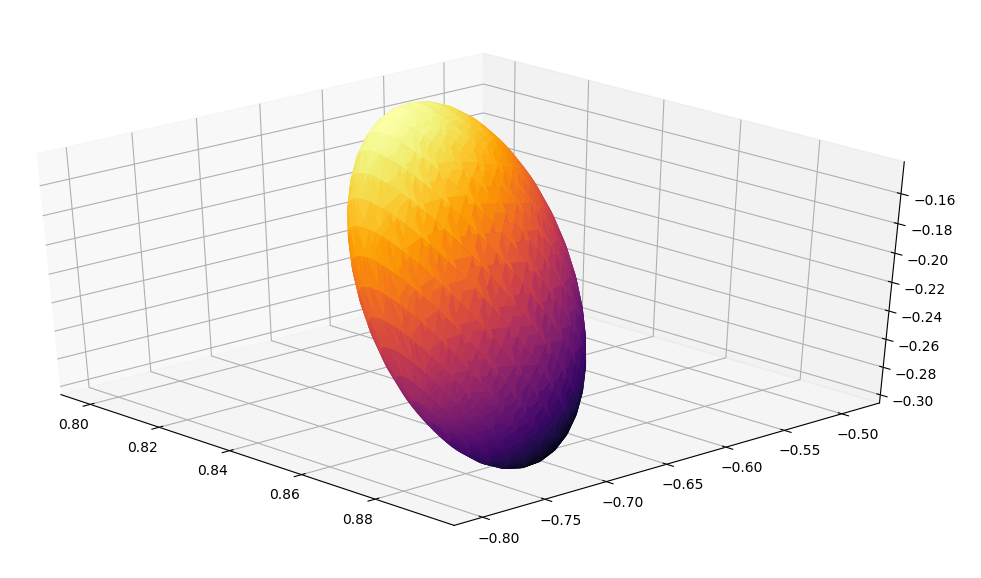
\includegraphics[width=16cm]{graphics/ConfidenceElipsoid1.png}
\caption{Elipsoid zaupanja za $\beta$, realiziran na naših podatkih.}
\end{figure}
\end{center}

\subsubsection{}
Za $\beta_j$ imamo sedaj intervale zaupanja stopnje zaupanja $1 - \alpha / m$ oblike
$$I_j := \left[\hat{\beta}_j \mp t_{n-m;\alpha/(2m)} \norm{y - \hat{y}}_2 \sqrt{((X^TX)^{-1})_{(j,j)} / (n-m)}\right].$$
Z Bonferonijevim popravkom dobimo, da je
$$I := \bigtimes_{j=1}^m I_j$$
kvader zaupanja s stopnjo $\alpha$. Na našem vzorcu imamo
$$I = [0.805, 0.887] \times [-0.778, -0.511] \times [-0.291, -0.154].$$
Na sliki vidimo, da je volumen kvadra zaupanja veliko večji od elipsoida in da prvi skoraj vsebuje drugega.
\begin{center}
\begin{figure}[h]
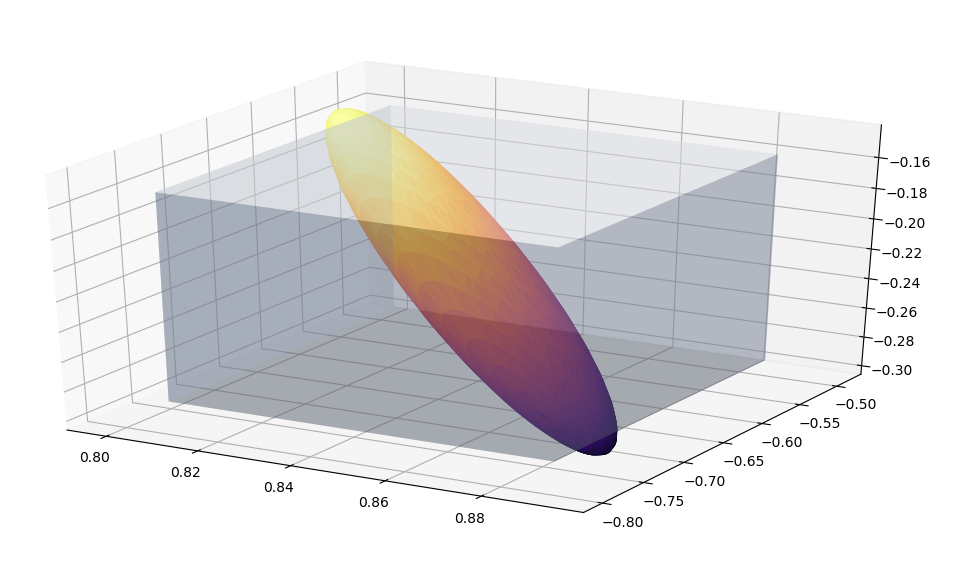
\includegraphics[width=16cm]{graphics/ConfidenceElipsoidVsCuboid1.png}
\caption{Kvader zaupanja in elipsoid zaupanja za $\beta$, realizirana na naših podatkih.}
\end{figure}
\end{center}

\section{}
\subsection{}
Vemo, da ima slučajna spremenljivka $Y$ Lebesguevo gostoto natanko tedaj, ko obstaja Borelova funkcija $f_Y \colon \R \to \R$, za katero velja
$$P(Y \leq y) = \int_{(-\infty, y]} f_Y d\LL = \int_{-\infty}^y f_Y(x) dx.$$
Upoštevamo izrek o popolni verjetnosti in Tonellijev izrek za zamenjavo vrstnega reda integracije, da dobimo
\begin{equation*}
\begin{aligned}
P(Y + Z \leq w) &= \sum_{z_k} P(Y \leq w - z_k) P(Z = z_k) = \sum_{z_k} \int_{-\infty}^{w-z_k} f_Y(y) P(Z = z_k) dy \\
&= \sum_{z_k} \int_{-\infty}^w f_Y(x - z_k) P(Z = z_k) dx = \int_{-\infty}^w \sum_{z_k} f_Y(x-z_k) P(Z = z_k) dx = \int_{-\infty}^w f_X(x) dx.
\end{aligned}
\end{equation*}
Ker je $(x,z_k) \mapsto f_Y(x - z_k) P(Z = z_k)$ merljiva in vrsta konvergentna za vsak $x\in\R$ (je dominirana z $1$), je $f_X \in B_\R / B_\R$ (po enem od izrekov teorije mere). Zato je $f_X$ Lebesgueva gostota slučajne spremenljivke $X = Y + Z$.

\subsection{}
Za $x\geq0$ dobimo
\begin{equation*}
\begin{aligned}
&f_X(x) = \sum_{k=0}^\infty \frac{c_k\lambda^k}{c(\lambda)}  \alpha (x-k)^{\alpha-1} \ind_{(0,1)}(x-k) 
= \frac{\alpha c_{\floor{x}}}{c(\lambda)} \lambda^{\floor{x}} (x-\floor{x})^{\alpha-1}, \\
&\ln(f_X(x)) = \ln(\alpha/c(\lambda)) + \ln(c_{\floor{x}}) + \floor{x}\ln(\lambda) + (\alpha-1)\ln(x - \floor{x}).
\end{aligned}
\end{equation*}

\subsection{}
Izrazimo
\begin{equation*}
f_{(X_1, \dots, X_n)}(x_1, \dots, x_n) = \left(\frac{\alpha}{c(\lambda)}\right)^n \left(\prod_{i=1}^n c_{\floor{x_i}}\right)
\exp\left(\adjscalar{\left[\ln(\lambda), \alpha-1\right], \left[\sum_{i=1}^n \floor{x_i}, \sum_{i=1}^n \ln(x_i - \floor{x_i})\right]}\right).
\end{equation*}
Po Fisher-Neymanovem izreku dobimo zadostnost statistike 
$$T(x_1, \dots, x_n) = \sum_{i=1}^n (\floor{x_i}, \ln(x_i - \floor{x_i})),$$
ker pa imamo eksponentni model s polnim rangom, sledi še, da je ta statistika tudi zadostna. Pripomnimo, da je verjetnost dogodka $\{X_i = \floor{X_i}\}$ enaka nič in da sta $T$ in $x \mapsto \prod_{i=1}^n c_{\floor{x_i}}$ Borelovi, saj ju lahko zapišemo kot vrsto konstantno pomnoženih indikatorjev (po predpostavki pa je slednja še nenegativna).

\end{document}